\subsection{Curves and Points}
\label{sec:implementation_curves}

OpenECC implements only curves of the simple Weierstrass form, internally known as \verb+WeierstrassCurve+s,
but is open to implementing different types of curves in the future.

Each curve implementation (implementing the \verb+ICurve+ interface) must have its own point implementation
(implementing the \verb+Point+ abstract class). A curve describes both the properties of the curve itself and
the properties used for encryption.

The simple Weierstrass curve describes the parameters \(a\) and \(b\) in the curve \(y^2 = x^3 + ax + b\), but
also the prime \(p\) of the prime field \(\mathbb{F}_p\) the curve is defined over; the generator point of the
curve; and the order of the generator point.

For each curve, the most basic point arithmetic must be implemented. This is limited to addition and negation, as
subtraction is implemented as negation-then-addition (\verb|p + (-q)|), and multiplication is implemented by the
multipliers (see the next section). This arithmetic is implemented in a class inheriting from \verb+Point+.

\begin{figure}[htb]
	\centering
	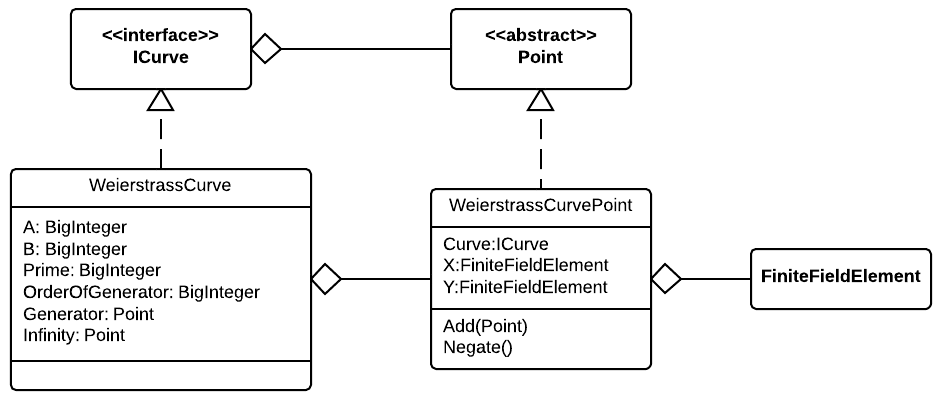
\includegraphics[width=1\textwidth]{implementation/curves}
	\caption{An example of the constructs that must be implemented in order to support a curve. On each class
		(\texttt{WeierstrassCurve} and \texttt{WeierstrassCurvePoint}) the methods and properties
		that are implemented are shown. The \texttt{BigInteger}s \texttt{A} and \texttt{B} on the curve are
		the curve parameters specific for this type of curve, and may vary from curve to curve. For example,
		an Edwards curve \(E_{edwards} : x^2 + y^2 = c^2 (1 + dx^2 y^2)\) is described by parameters known as
        \texttt{C} and \texttt{D}.}
\end{figure}

The \verb+Point+ abstract class provides a concise syntax that is close to the natural mathematical syntax used
when discussing ECC (especially evident when compared with, for example, the syntax of BouncyCastle), overriding
operators to make the syntax look natural: \verb|p + q| instead of \verb|p.Add(q)|, and \verb|p + (q - r)| instead of
\verb|p.Add(q.Subtract(r))|.

Instead of requiring the user of the library to know of safe curve parameters, some well-known curves have been
provided through the \verb|CurveFactory|. While only Weierstrass curves -- which are not necessarily
safe\footnote{All known Weierstrass curves have some issues regarding safety, leaking information through timing
attacks, their points being distinguishable from truly random strings, etc.\cite{safecurves}} -- are supported, and no real
guarantee of security can be made, this approach discourages experimentation, and the resulting unsafe curves.

Custom curves can still be constructed through the constructors of the curve implementations.

\begin{figure}
	
\end{figure}